\documentclass{article}

\usepackage{fancyhdr}
\usepackage{extramarks}
\usepackage{amsmath}
\usepackage{amssymb}
\usepackage{enumerate}
\usepackage{graphicx}
\usepackage{pgfplotstable}

%
% Basic Document Settings
%

\topmargin=-0.45in
\evensidemargin=0in
\oddsidemargin=0in
\textwidth=6.5in
\textheight=9.0in
\headsep=0.25in

\linespread{1.1}

\pagestyle{fancy}
\lhead{\hmwkAuthorName}
\chead{\hmwkClass\ : \hmwkTitle}
\rhead{\firstxmark}
\lfoot{\lastxmark}
\cfoot{\thepage}

\renewcommand\headrulewidth{0.4pt}
\renewcommand\footrulewidth{0.4pt}

\setlength\parindent{0pt}

%
% Create Problem Sections
%

\newcommand{\enterProblemHeader}[1]{
    \nobreak\extramarks{}{Problem \arabic{#1} continued on next page\ldots}\nobreak{}
    \nobreak\extramarks{Problem \arabic{#1} (continued)}{Problem \arabic{#1} continued on next page\ldots}\nobreak{}
}

\newcommand{\exitProblemHeader}[1]{
    \nobreak\extramarks{Problem \arabic{#1} (continued)}{Problem \arabic{#1} continued on next page\ldots}\nobreak{}
    \stepcounter{#1}
    \nobreak\extramarks{Problem \arabic{#1}}{}\nobreak{}
}

\setcounter{secnumdepth}{0}
\newcounter{partCounter}
\newcounter{homeworkProblemCounter}
\setcounter{homeworkProblemCounter}{1}
\nobreak\extramarks{Problem \arabic{homeworkProblemCounter}}{}\nobreak{}

%
% Homework Problem Environment
%
% This environment takes an optional argument. When given, it will adjust the
% problem counter. This is useful for when the problems given for your
% assignment aren't sequential. See the last 3 problems of this template for an
% example.
%
\newenvironment{homeworkProblem}[1][-1]{
    \ifnum#1>0
        \setcounter{homeworkProblemCounter}{#1}
    \fi
    \section{Problem \arabic{homeworkProblemCounter}}
    \setcounter{partCounter}{1}
    \enterProblemHeader{homeworkProblemCounter}
}{
    \exitProblemHeader{homeworkProblemCounter}
}

%
% Homework Details
%   - Title
%   - Due date
%   - Class
%   - Section/Time
%   - Instructor
%   - Author
%

\newcommand{\hmwkTitle}{Homework\ \#5}
\newcommand{\hmwkDueDate}{February 24, 2015}
\newcommand{\hmwkClass}{PHYS 5243 - Solid State Physics}
\newcommand{\hmwkClassInstructor}{Professor Sheena Murphy}
\newcommand{\hmwkAuthorName}{Chase Brown}


\begin{document}
	\begin{homeworkProblem}
		\textbf{Simon - Solid State Basics - Problem 10.1: Normal Modes of a One-Dimensonal Diatomic Chain}
		\hfill
		\begin{enumerate}[(a)]
			\item What is the difference between an acoustic mode and an optical mode? 
				\begin{itemize}
					\item Describe how the particles move in each case.
				\end{itemize}
			\item Derive the dispersion relation for the longitudinal oscillations of a one-dimensional diatomic mass-and-spring crystal where the unit cell is of length $a$ and each unit cell contains one atom of mass $m_1$ and one atom of mass $m_2$ connected together by springs with spring constant $\kappa$, as shown in the figure (all springs are the same, and motion of particles is in one dimension only).
			\\
			\centerline{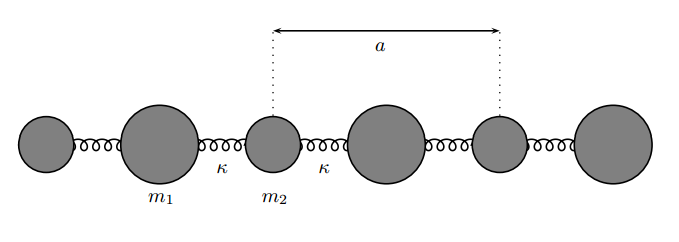
\includegraphics[scale=0.7]{mass_spring.png}}
			\\
			\item Determine the frequences of the acoustic and optical modes at $k=0$ as well as the Brillouin zone boundary.
				\begin{itemize}
					\item Describe the motion of the masses in each case. (Margin note 4 in Chapter 10 of Simon's Solid State Basics) 
					\item Determine the sound velocity and show that the group velocity is zero at the zone boundary.
					\item Show that the sound velocity is also given by $v_s=\sqrt{\frac{1}{\beta \rho}}$, where $\beta$ is the compressibility.
				\end{itemize}
			\item Sketch the dispersion in both reduced and extended zone scheme.
				\begin{itemize}
					\item If there are $N$ unit cells, how many different normal modes are there?
					\item How many \textit{branches} of excitations are there? In other words, in the reduced zone scheme, how many modes are there at each $k$?
				\end{itemize}
			\item What happens when $m_1 = m_2$?
		\end{enumerate}

		\textbf{Solution}
			\begin{enumerate}[(a)]
				\item Optical phonon modes occur when each neighboring atom within the lattice is out of phase with the atom considered. Acoustic phonon modes occur when all of the atoms within the lattice are in phase (on the same wave).  The image below provides a description of how these two phonon modes appear in real space.  The optical modes are typically excited by energies within the visible region of light ($\sim$ 1-3 $eV$), which is a much larger energy than that required for acoustic phonon modes.
					\centerline{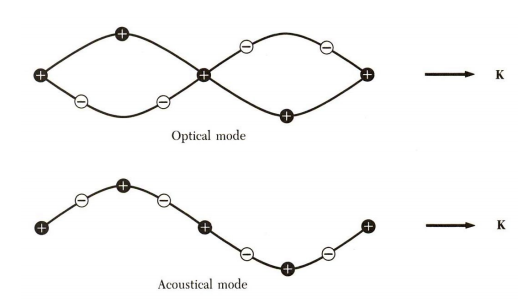
\includegraphics[scale=0.8]{Acoustic_optical.png}}
				
				\item Starting with versions of equations 10.1 and 10.2 from Simon's Solid State Basics adapted for different masses and same spring cosntants:
					\begin{equation*}
						\begin{aligned}
							m_1 \ddot{\delta x_n} = \kappa (\delta y_n - \delta x_n) + \kappa (\delta y_{n-1} - \delta x_n) \\
							m_2 \ddot{\delta y_n} = \kappa (\delta x_{n+1} - \delta y_n) + \kappa (\delta x_n - \delta y_n)
						\end{aligned}
					\end{equation*}
					Which gives us the equations of motion as:
					\begin{equation*}
						\begin{aligned}
							m_1 \ddot{\delta x_n} = \kappa (\delta y_n + \delta y_{n-1} - 2 \delta x_n) \\
							m_2 \ddot{\delta y_n} = \kappa (\delta x_{n+1} + \delta x_n - 2\delta y_n)
						\end{aligned}
					\end{equation*}

					We then assume this can be viewed as a wave:	
						\begin{equation*}
							\begin{aligned}
								\delta x_n = A_x e^{i(qna-\omega t)} \\
								\delta y_n = A_y e^{i(qna-\omega t)}
							\end{aligned}
						\end{equation*}
					Therefore we have :
						\begin{equation*}
							\begin{aligned}
								m_1 \omega^2 A_x e^{i(qna-\omega t)} = \kappa (A_y e^{i(qna-\omega t)} - A_x e^{i(qna-\omega t)}) + \kappa (A_y e^{i(q(n-1)a-\omega t)} - A_x e^{i(qna-\omega t)}) \\
								m_2 \omega^2 A_y e^{i(qna-\omega t)} = \kappa (A_x e^{i(q(n+1)a-\omega t)} - A_y e^{i(qna-\omega t)}) + \kappa (A_x e^{i(qna-\omega t)} - A_y e^{i(qna-\omega t)})
							\end{aligned}
						\end{equation*}

						\begin{equation*}
							\begin{aligned}
								\Rightarrow m_1 \omega^2 A_x = \kappa (A_y  - A_x + A_y e^{ika} - A_x ) \\
											m_2 \omega^2 A_y = \kappa (A_x e^{-ika} - A_y + A_x - A_y ) 
							\end{aligned}
						\end{equation*}

						\begin{equation*}
							\begin{aligned}
								\Rightarrow m_1 \omega^2 A_x = \kappa (A_y (1+e^{ika}) - 2A_x ) \\
											m_2 \omega^2 A_y = \kappa (A_x (1+e^{ika}) - 2A_y ) 
							\end{aligned}
						\end{equation*}

						\begin{equation*}
							\Rightarrow m_1 \omega^2 \left| \begin{array}{c} 
																A_x \\
																A_y \end{array} \right|  =  
																	\left| \begin{array}{cc} 
																		-2\kappa & \kappa(1+e^{ika}) \\
																		\kappa(1+e^{ika}) & -2\kappa \end{array} \right| 
																			\left| \begin{array}{c} 
																					A_x \\
																					A_y \end{array} \right| 
						\end{equation*}
					Now take the determinant:
						\begin{equation*}
							0 = \left| \begin{array}{cc} 
									-2\kappa & \kappa(1+e^{ika}) \\
									\kappa(1+e^{ika}) & -2\kappa \end{array} \right| 
										\left| \begin{array}{c} 
												A_x \\
												A_y \end{array} \right| 
						\end{equation*}

			\end{enumerate}


	\end{homeworkProblem}


\end{document}
